\chapter{REFERENCIAL TEÓRICO}
\label{cap:elementos}

Durante o estágio, vários novos conceitos e expressões me foram ensinados, pois estes mesmos termos seriam recorrentes em meu cotidiano.

Devido ao grande número de termos específicos da área de desenvolvimento, faz-se necessária a explicação dos mesmos.

\section{Metodologias Ágeis}

São estratégias e comportamentos que devem ser seguidos afim de obter um resultado otimizado e mensurável.

\subsection{Scrum}

Metodologia ágil que visa ter escopo fechado (número de tarefas predefinidas), calculadas através de métricas da equipe, como pontos de esforço.

Muitas vezes separadas em Sprints (tempo pré-definido pela equipe, geralmente de 10 dias úteis), as tarefas são incluídas em um quadro e devem ser finalizadas no prazo previsto..
\begin{quote}
  Scrum é um framework simples e pequeno e, assim, funciona bem em  cada contexto se for utilizado em conjunto com outras técnicas e praticas a serem experimentadas e adaptadas. - \cite{sabbagh2014scrum}
\end{quote}
\begin{quote}
  O sprint é o ciclo de desenvolvimento, onde o incremento do produto pronto é gerado pelo Time de Desenvolvimento a partir dos itens mais importantes do Product Backlog. - \cite{sabbagh2014scrum}
\end{quote}

\subsection{Kanban}
  Opção de metodologia ágil mais adaptativa, tendo escopo aberto torna-se possível inserir atividades durante o tempo.
  Geralmente é determinado um máximo de esforço e, ao final de uma atividade, é inserida uma nova com prioridade.

  \begin{quote}
    O kanban, ou mais precisamente o "sistema Kanban para desenvolvimento de software" representa uma implementação mais direta dos princípios de Desenvolvimento Lean de Produtos para o desenvolvimento de software que os métodos aágeis tradicionais. Com foco consistente no fluxo e no contexto, o Kanban oferece uma abordagem menos prescritiva comparada ao Agile, e tem se tornado uma extensão popular dos métodos ágeis tradicionais como Scrum e XP. - \cite{boeg2010kanban}
  \end{quote}
\begin{figure}[H]
\centering
\caption{Quadro kanban} %legenda
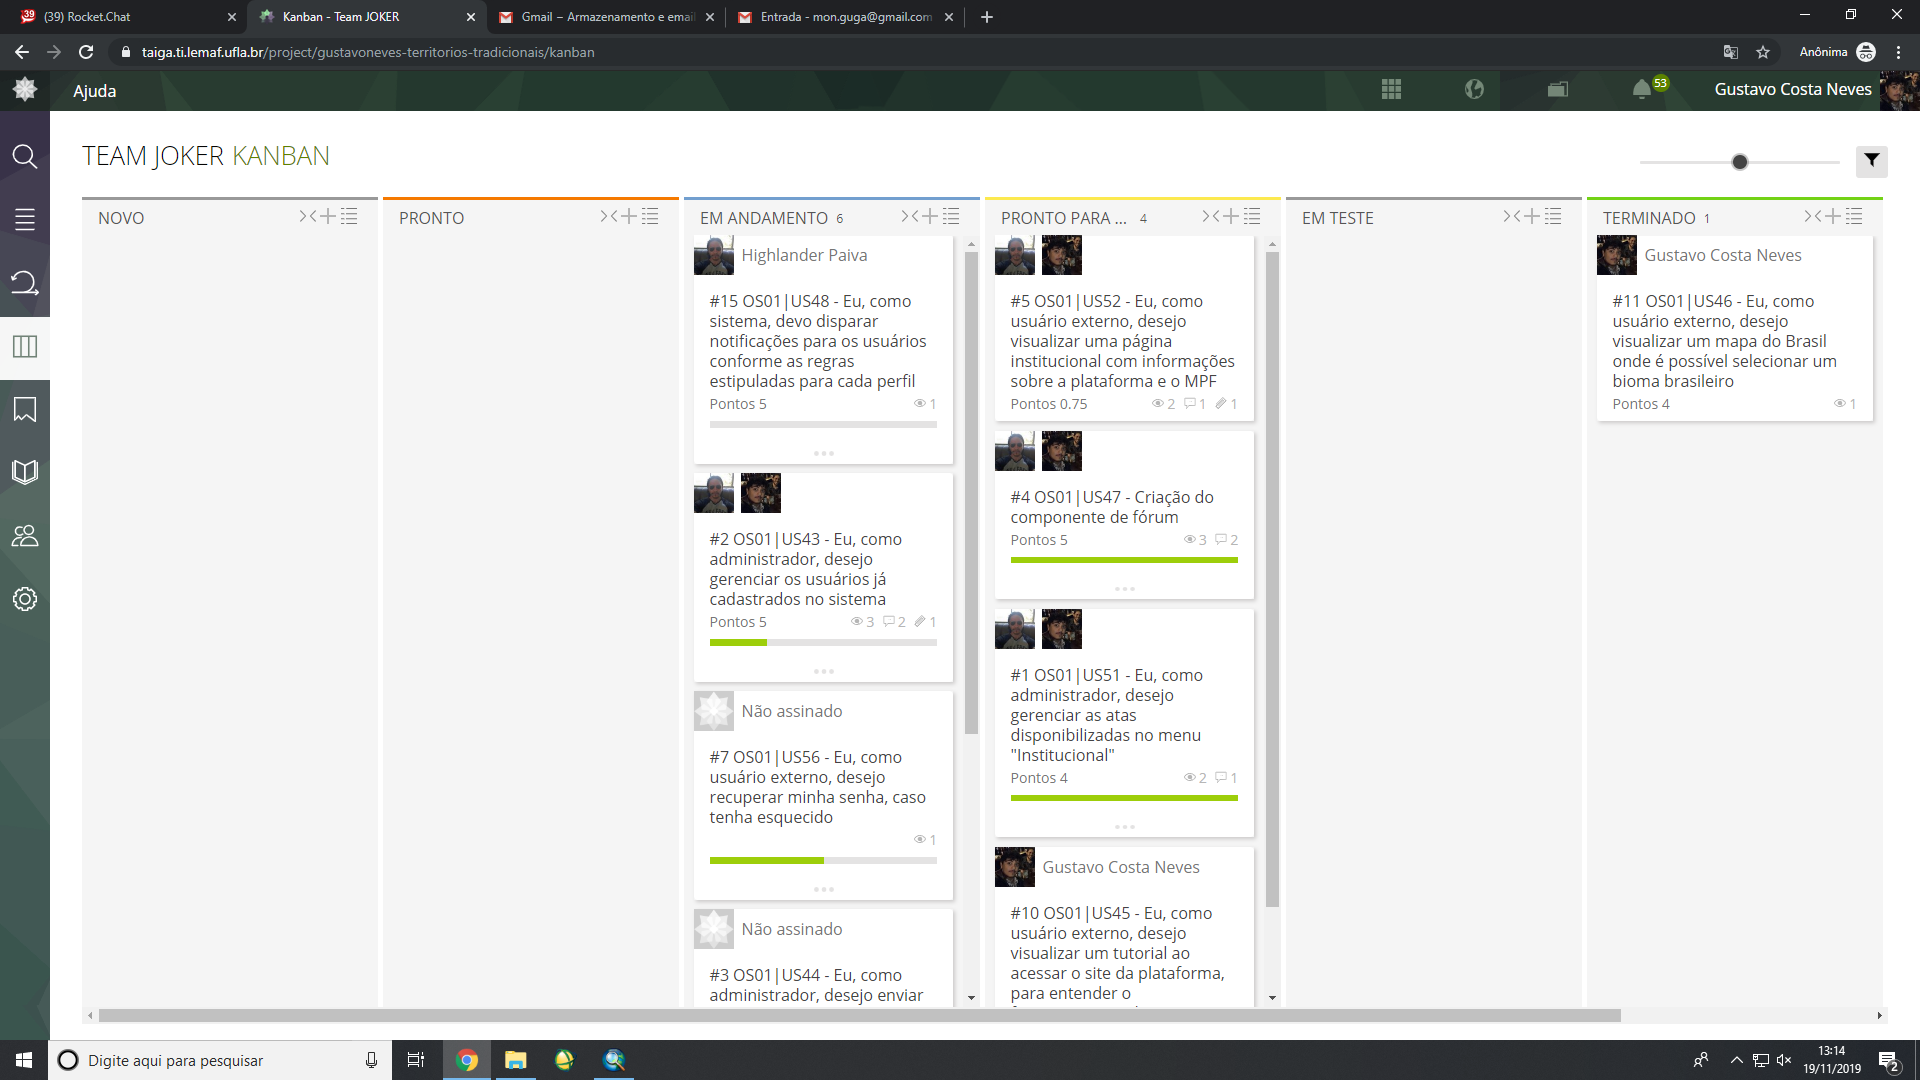
\includegraphics[scale=0.2]{quadroKanban}\\  % o 0.9 indica 90% do tamanho original
% pdfLaTeX aceita figuras no formato PNG, JPG ou PDF
% figuras vetoriais podem ser exportadas para eps e depois convertidas para pdf usando epstopdf
{\small Fonte: https://taiga.ti.LEMAF.ufla.br/} %Fonte da imagem
\label{fig:exemplo} %rotulo para refencia
\end{figure}

\section{Frameworks}

Para facilitar o desenvolvimento, diversas ferramentas foram criadas e durante o desenvolvimento de novos projetos foi necessária a utilização das mesmas.

\subsection{Frontend}

É a parte da aplicação que interage diretamente com o usuário.

\subsubsection{Angular}

Angular é um framework open-source, de desenvolvimento front-end, que possibilita o desenvolvimento de aplicações web.

Teve sua primeira versão lançada em 2016.

\begin{quote}
  o AngularJS foi criado por Miško Hevery e Adam Abron  em  2009  e  é  um  framework  JavaScript open  source(código  aberto), client-side(do lado  do  cliente)  que  promove  uma  alta  produtividade  na  experiência  do  desenvolvimento Web - \cite{ferreira2018analise}
\end{quote}


\subsubsection{VueJS}

Vue.js é um framework JavaScript de open-source, focado no desenvolvimento de interfaces de usuário e aplicativos de página única.

Teve sua primeira versão lançada em 2014.

\begin{quote}
  Vue é uma lib/framework JavaScript reativo, para  o  desenvolvimento  de  componentes  que,  por  sua  vez,  são  códigos  que  podem  ser reaproveitados em sua aplicação - \cite{ferreira2018analise}
\end{quote}


\subsubsection{ReactJS}

O React é uma biblioteca JavaScript, open-source, com foco em criar interfaces de usuário em páginas web. É mantido por empresas como Facebook e Instagram e uma comunidade de desenvolvedores individuais. 

Teve sua primeira versão lançada em 2013.

\begin{quote}
  Segundo a sua documentação(2018), ele é, na  verdade,  uma  biblioteca  de  UI  (User  Interface),  representando  apenas  a  camada viewdoModel  View  Controler(MVC).  - \cite{ferreira2018analise}
\end{quote}

\subsection{Backend}

É a parte da aplicação que é inacessível ao usuário, onde é controlado todo o sistema (autenticação, regras de negocio, jobs e etc).

\subsubsection{PlayFramework}

O Play Framework é uma alternativa "limpa" de esticar as stacks do Java Enterprise. Ele se concentra na produtividade do desenvolvedor e tem como objetivo arquiteturas RESTful. 

O objetivo da estrutura do Play é facilitar o desenvolvimento de aplicativos da web, mantendo o Java.

Teve sua primeira versão lançada em 2009.

\begin{quote}
Play! Framework 2 é planejado para ser "full stack" e completamente integrada, a boa notícia é que não há requisitos específicos para você ou seu ambiente começar a criar novos aplicativos da web. - \cite{petrella2013learning}
\end{quote}

\subsubsection{Spring Boot}

O Spring é um framework open-source para a plataforma Java criado por Rod Johnson e descrito em seu livro "Expert One-on-One: JEE Design e Development".
Trata-se de um framework baseado nos padrões de projeto inversão de controle e injeção de dependência.

Teve sua primeira versão em 2002.

\begin{quote}
  Spring Framework é um framework voltado para desenvolvimento de aplicações corportaivas para a plataforma Java, baseado nos conceitos de inversão de controle e injeção de dependencias. - \cite{weissmann2014vire}
\end{quote}

\subsubsection{DotNet Framework}

O .NET Framework é uma iniciativa da empresa Microsoft, que visa uma plataforma única para desenvolvimento e execução de sistemas e aplicações.
Todo e qualquer código gerado para .NET pode ser executado em qualquer dispositivo que possua um framework de tal plataforma.

Teve sua primeira versão lançada em 2002.

\begin{quote}
  
O .Net Framework é um framework de desenvolvimento que fornece uma nova interface de programação para serviços e APIs do Windows e integra várias tecnologias que surgiram da Microsoft no final dos anos 90. \cite{thai2003net}
\end{quote}

\section{Cargos}

Para melhor organização dos projetos, os funcionários são separados em tribos, que são constituídas de squads, com cargos determinados a cada integrante.

\subsection{Scrum Master}

Cargo que tem como função cuidar das obrigações impostas sobre a metodologia scrum, como lembrar dos ritos, marcar reuniões e garantir o bom desenvolvimento das atividades estabelecidas para a sprint.

\subsection{Gerente de projetos(GP)}

Cargo que tem como função gerenciar os projetos e times da sua
 tribo, cuidando para que sejam entregues os requisitos no prazo combinado.

\subsection{Product Owner(PO)}
Cargo que tem como função cuidar do relacionamento do time com o produto,
 definindo e priorizando requisitos.
 